%-----------------------------------------------------------------------
\chapter{Results}
In this chapter we shall introduce our final results, highlight the strengths and weaknesses, and compare the results we have produced throughout the course of this project.

In general, our final animation well resembles the motion of the actor, see Fig.~\ref{fig:results1}. The animation runs at $60$ frames per second, it is smooth and expressive, see the video in the supplementary material. The animation respects the intrinsic differences between the actor and Emily, i.e. the animated expressions are not exact replicas of the actor's expressions; instead they are Emily versions of the actor's expressions. The final result was enhanced by manually activating the blendshapes that control blinks and winks throughout the motion sequence, see Fig.~\ref{fig:results2a}. Moreover, the head motion that we removed before solving for blendshape weights (see Sec.~\ref{sec:stabilising_head_movement}), was reintroduced to make the animation appear more dynamic, see Fig.~\ref{fig:results3}.

\begin{figure}
        \centering
        \begin{subfigure}[t]{0.43\textwidth}
                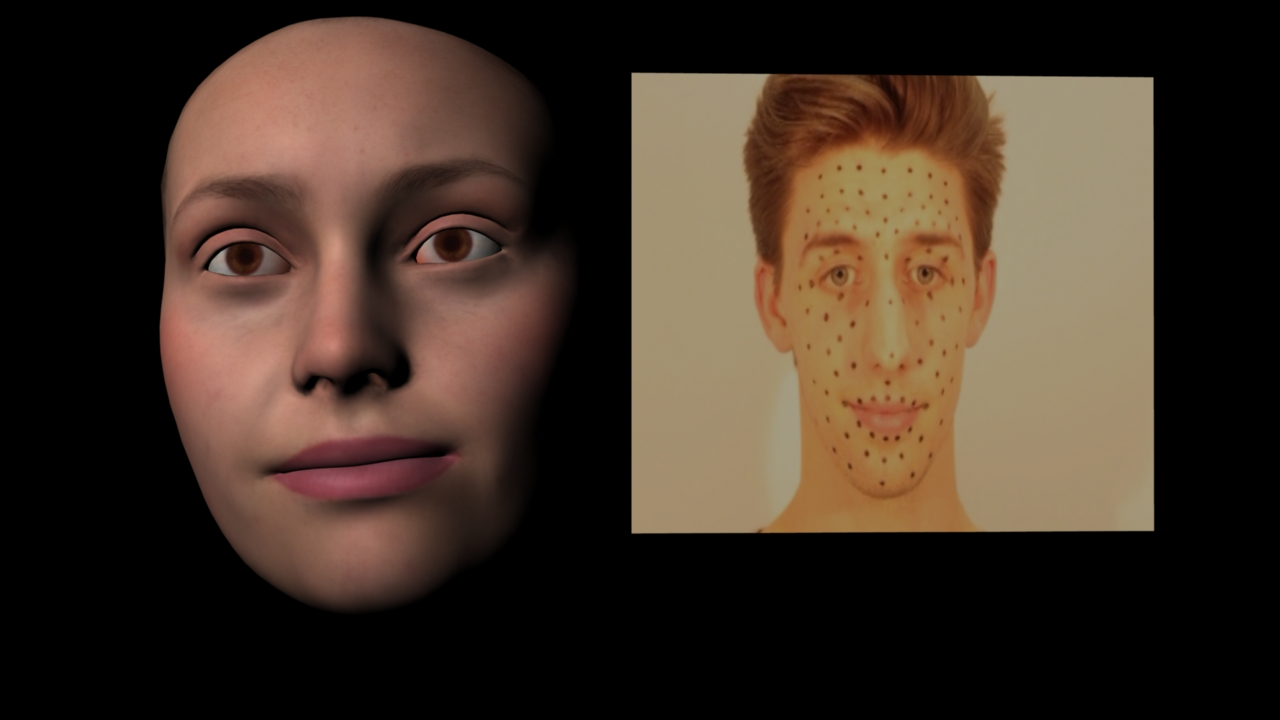
\includegraphics[width=\textwidth]{img/results/Emily_Maya_clean_video_300}
        \end{subfigure}
        \begin{subfigure}[t]{0.43\textwidth}
                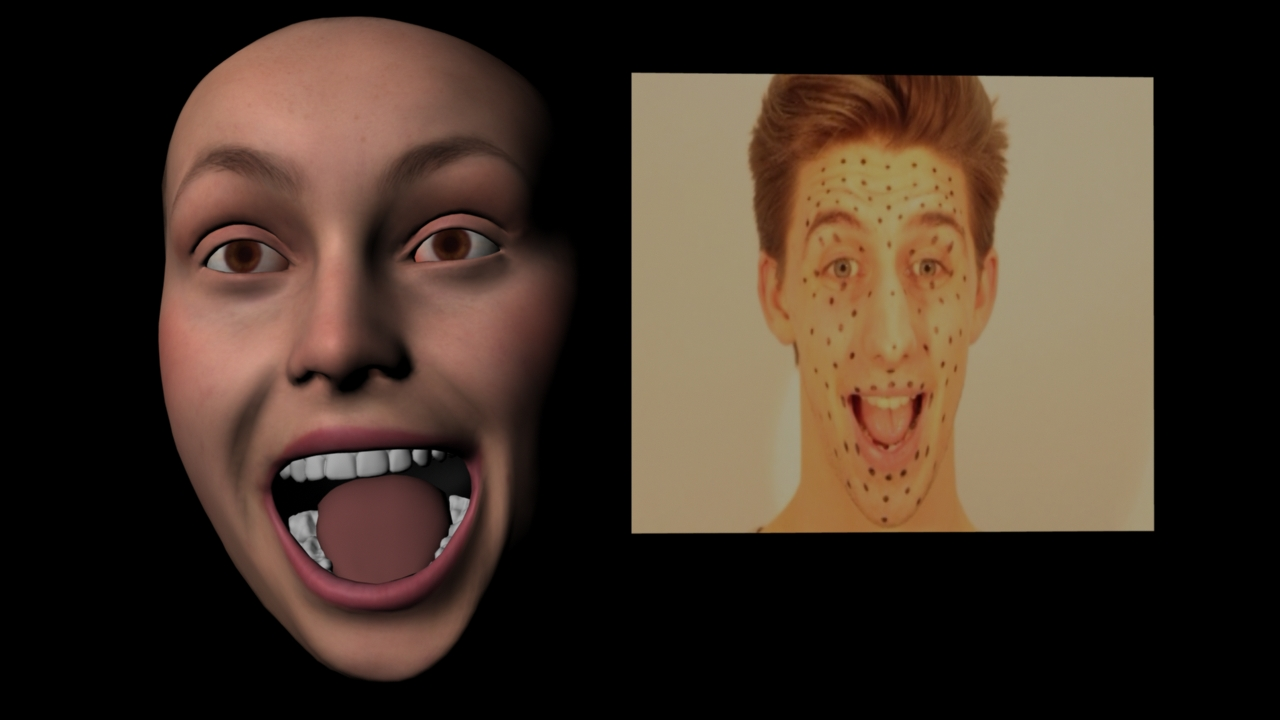
\includegraphics[width=\textwidth]{img/results/Emily_Maya_clean_video_1187}
        \end{subfigure}\\
        \begin{subfigure}[t]{0.43\textwidth}
                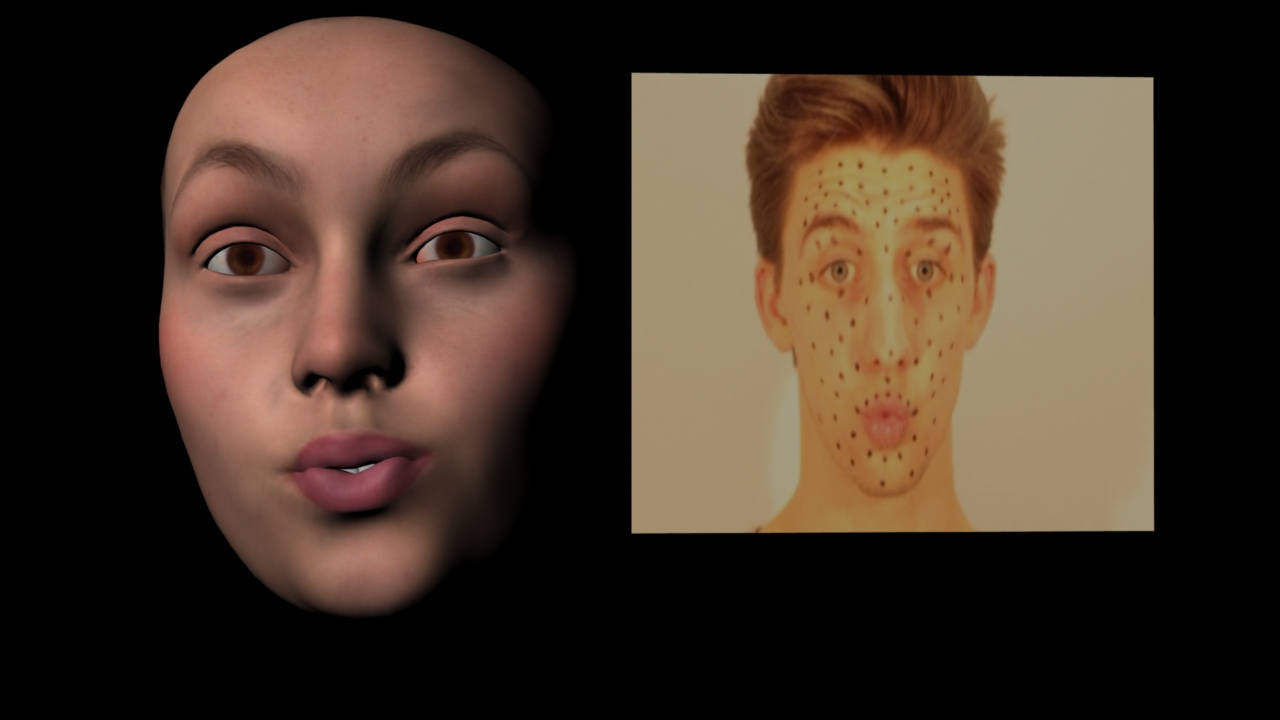
\includegraphics[width=\textwidth]{img/results/Emily_Maya_clean_video_1544}
        \end{subfigure}
        \begin{subfigure}[t]{0.43\textwidth}
                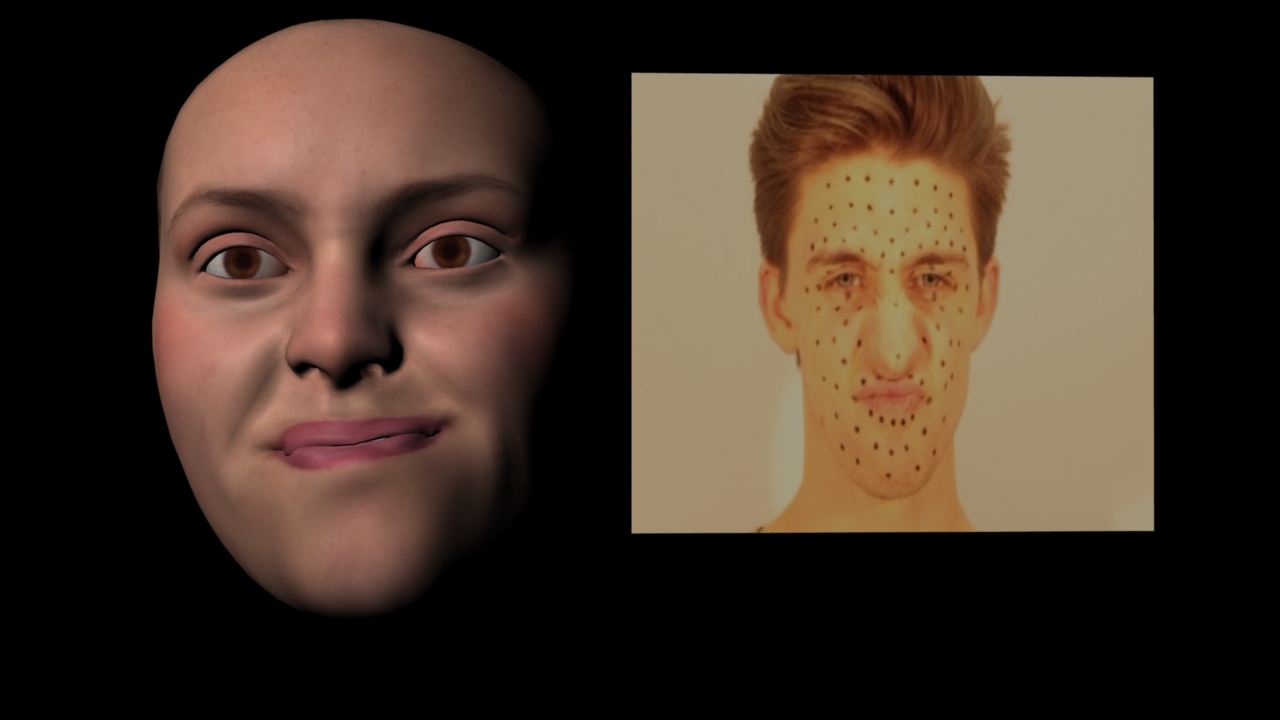
\includegraphics[width=\textwidth]{img/results/Emily_Maya_clean_video_2135}
        \end{subfigure}
        \caption{The final animation well resembles the captured sequence.}
        \label{fig:results1}
\end{figure}
\begin{figure}
        \centering
        \begin{subfigure}[t]{0.43\textwidth}
                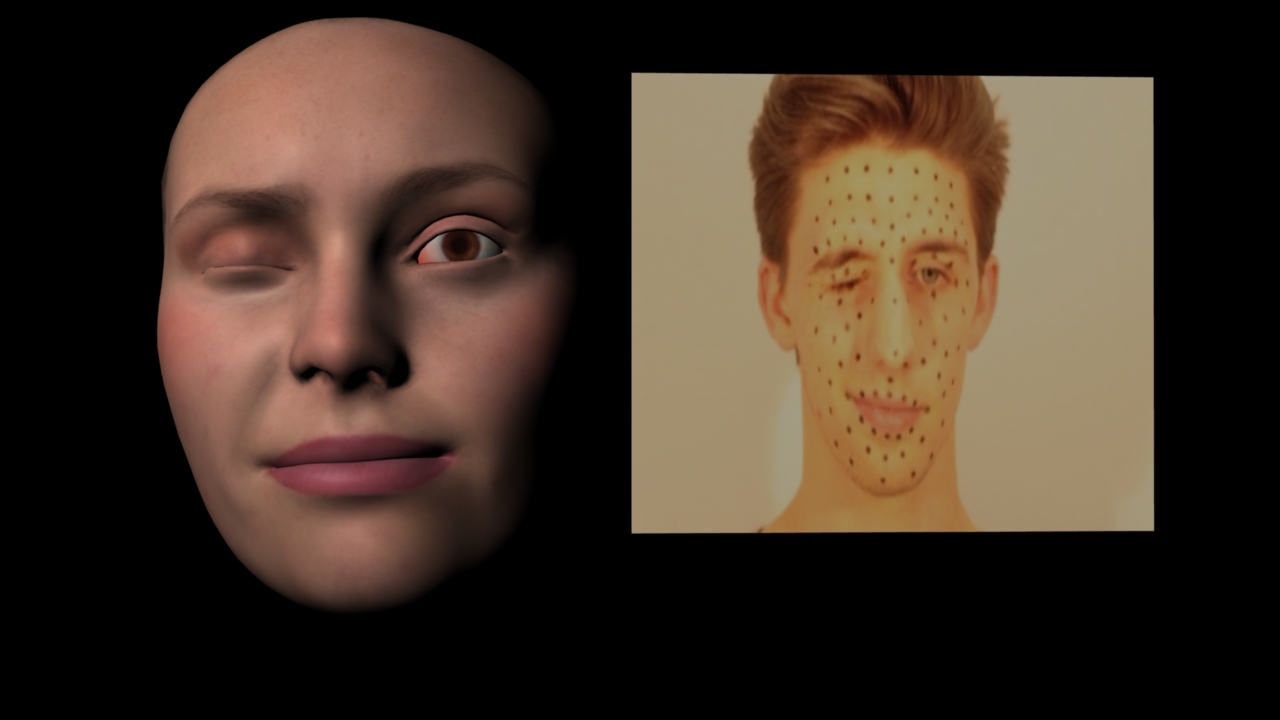
\includegraphics[width=\textwidth]{img/results/Emily_Maya_clean_video_775}
                \caption{Manually added blinks.}\label{fig:results2a}
        \end{subfigure}
        \begin{subfigure}[t]{0.43\textwidth}
                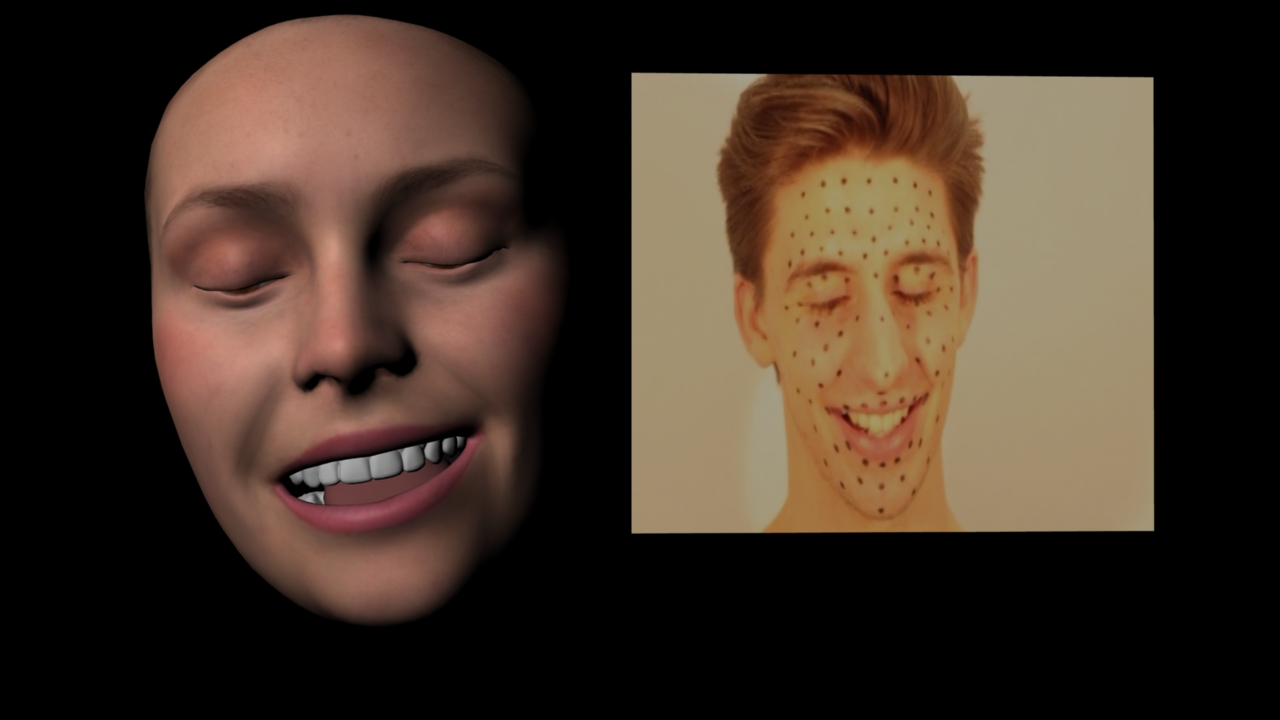
\includegraphics[width=\textwidth]{img/results/Emily_Maya_clean_video_2941}
                \caption{Reintroduced the head rotation.}
        \end{subfigure}
        \caption{Improvements to the blendshape model.}\label{fig:results2b}
        \label{fig:results2}
\end{figure}

The final animation has a number of flaws. First, since only a sparse set of points is used to find the blendshape weights, some motion remains poorly captured; Fig.~\ref{fig:results3a} presents such a situation. Here the sparse points alone are unable to define the downward positioning of the mouth; the markers around the mouth form a ellipse which is then replicated by Emily without taking into consideration the fact that the actor's mouth is shut. Another issue is visible in Fig.~\ref{fig:results3b}; here the spherical structure that represents the inside of the mouth is penetrating Emily's cheek. Unfortunately, we have no control over the motion of this inner structure, and it cannot be hidden since it is connected to the mesh of the face. Our approach to this problem involves limiting the upper bound on the weights to ensure that the combination of blendshapes that cause this problem does not occur; by trial and error we were able to eliminate most of the problematic mixtures of shapes.

\begin{figure}
        \centering
        \begin{subfigure}[t]{0.43\textwidth}
                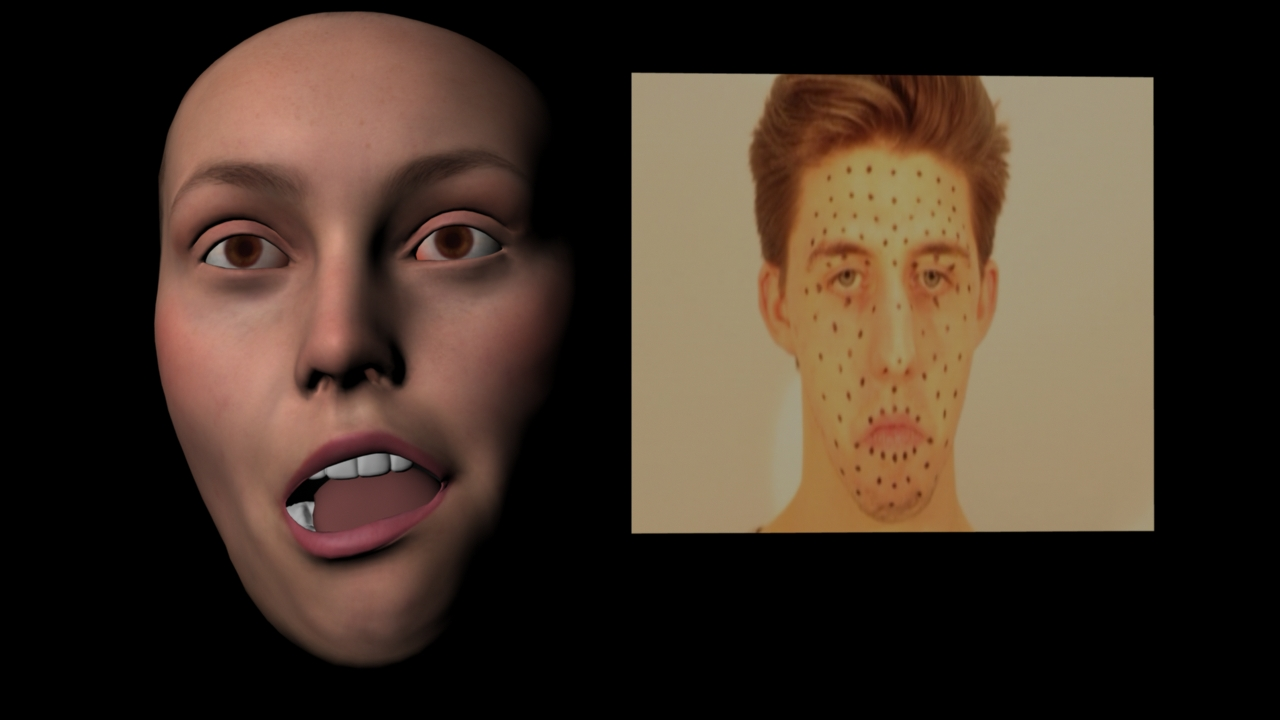
\includegraphics[width=\textwidth]{img/results/Emily_Maya_clean_video_2578}
        \caption{Sparse data does not describe the motion fully.}\label{fig:results3a}
        \end{subfigure}
        \begin{subfigure}[t]{0.43\textwidth}
                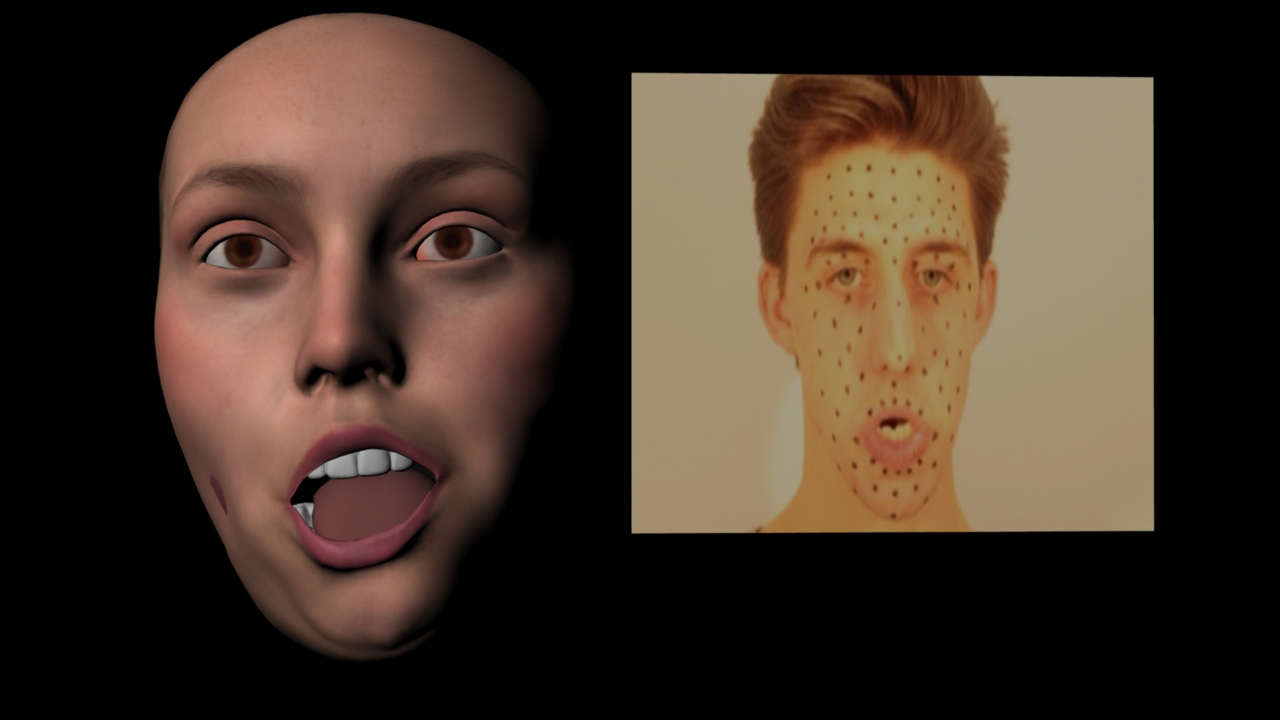
\includegraphics[width=\textwidth]{img/results/Emily_Maya_clean_video_2631}
		\caption{The mesh inside the mouth is allowed to penetrate itself.}\label{fig:results3b}        
        \end{subfigure}
        \caption{Shortcomings of the current model.}
        \label{fig:results3}
\end{figure}